\section{Evaluation}
\label{res_overview}

\begin{table*}[h]
    \centering\small\footnotesize
    \caption{Evaluation results overview. We evaluate two different versions of mbed TLS, five different
        versions of OpenSSL and Monocypher 3.0\@. CF represents secret-dependent control-flow transfers and
        DF represents secret-dependent data-flow transfers. A summary of vulnerabilities 
        with the amount of leaked information can be found in Appendix \S\ref{sec:result-table}.
    }\label{table:over_result}
    \vspace*{-9pt}
    \newlength{\x}
    \newlength{\y}
    \settowidth{\x}{~~}
    \settowidth{\y}{m}
    \addtolength{\x}{-1\y}
    \newcommand{\foo}{\mbox{\hspace*{\the\x}}}
%    \resizebox{1.9\columnwidth}{!}{

    \begin{tabular}{llrrrrrrr}
        \hline
        \textbf{Algorithm} & \textbf{Version}  & \textbf{Leakage Sites} & \textbf{CF}         & \textbf{DF}
                           & \textbf{\# Instructions} & \textbf{Max Leakage}   & \textbf{Sym.\ Exe.} & \textbf{Monte Carlo}                                                    \\\hline
                           &                          &                        &                     &                      &             & bits & ms        & ms              \\\cline{7-9}
        AES                & Mbed TLS 2.5             & 68                     & 0                   & 68                   & 39,855      & 8.6  & 512 ~~    & 1,052 ~~        \\
        AES                & Mbed TLS 2.15            & 68                     & 0                   & 68                   & 39,855      & 9.1  & 520 ~~    & 1,057 ~~        \\
        AES                & OpenSSL 0.9.7            & 75                     & 0                   & 75                   & 1,704       & 10.6 & 231 ~~    & 9,199 ~~        \\
        AES                & OpenSSL 1.0.2f           & 88                     & 0                   & 88                   & 1,350       & 12.0 & 36 ~~     & 1,924 ~~        \\
        AES                & OpenSSL 1.0.2k           & 88                     & 0                   & 88                   & 1,350       & 12.5 & 35 ~~     & 1,961 ~~        \\
        AES                & OpenSSL 1.1.0f           & 88                     & 0                   & 88                   & 1,420       & 12.6 & 36 ~~     & 2,161 ~~        \\
        AES                & OpenSSL 1.1.1            & 88                     & 0                   & 88                   & 1,586       & 4.4  & 43 ~~     & 1,631 ~~        \\
        DES                & Mbed TLS 2.5             & 15                     & 0                   & 15                   & 4,596       & 1.1  & 58 ~~     & 162 ~~          \\
        DES                & Mbed TLS 2.15            & 15                     & 0                   & 15                   & 4,596       & 1.0  & 57 ~~     & 162 ~~          \\
        DES                & OpenSSL 0.9.7            & 6                      & 0                   & 6                    & 2,976       & 7.6  & 163 ~~    & 4,677       ~~  \\
        DES                & OpenSSL 1.0.2f           & 8                      & 0                   & 8                    & 2,593       & 9.8  & 166 ~~    & 6,509       ~~  \\
        DES                & OpenSSL 1.0.2k           & 8                      & 0                   & 8                    & 2,593       & 10.1 & 165 ~~    & 5,975        ~~ \\
        DES                & OpenSSL 1.1.0f           & 8                      & 0                   & 8                    & 4,260       & 8.8  & 182 ~~    & 5,292        ~~ \\
        DES                & OpenSSL 1.1.1            & 6                      & 0                   & 6                    & 8,272       & 7.5  & 229 ~~    & 5,152       ~~  \\
                           &                          &                        &                     &                      &             &      & seconds   & seconds               \\\cline{8-9}
        Chacha20           & Monocypher 3.0           & 0                      & 0                   & 0                    & 149,353     & 0    & 2 ~~    & 0           ~~  \\  
        Poly1305           & Monocypher 3.0           & 0                      & 0                   & 0                    & 1,213,937   & 0    & 15 ~~   & 0           ~~  \\
        Argon2i            & Monocypher 3.0           & 0                      & 0                   & 0                    & 4,595,142   & 0    & 37 ~~   & 0           ~~  \\
        Ed25519              & Monocypher 3.0           & 0                      & 0                   & 0                    & 5,713,619   & 0    & 271 ~~  & 0           ~~  \\
                           &                          &                        &                     &                      &             &      & minutes   & minutes         \\\cline{8-9}
        RSA                & Mbed TLS 2.5             & 6                      & 6                   & 0                    & 22,109,246  & 9.6  & 39 ~~     & 41  ~~          \\
        RSA                & Mbed TLS 2.15            & 12                     & 12                  & 0                    & 24,484,441  & 8.7  & 44 ~~     & 251  ~~         \\
        RSA                & OpenSSL 0.9.7            & 107                    & 105                 & 2                    & 17,002,523  & 17.2 & 23 ~~     & 428 ~~          \\
        RSA                & OpenSSL 1.0.2f           & 38                     & 27                  & 11                   & 14,468,307  & 16.2 & 29 ~~     & 436  ~~         \\
        RSA                & OpenSSL 1.0.2k           & 36                     & 27                  & 9                    & 15,285,210  & 14.2 & 40 ~~     & 714   ~~        \\
        RSA                & OpenSSL 1.1.0f           & 31                     & 22                  & 9                    & 16,390,750  & 17.2 & 34 ~~     & 490 ~~          \\
        RSA                & OpenSSL 1.1.1            & 27                     & 20                  & 7                    & 18,207,020  & 14.9 & 7 ~~      & 501 ~~          \\
        Total              &                          & 886                    & 219                 & 667                  & 139,733,961 &      & 214m \foo & 2,861m \foo     \\\hline
        %                    &                          &                       &                     &                      &             & bits & ms        & ms              \\\cline{7-9}
        % AES                & Mbed TLS 2.5             & 68                    & 0                   & 68                   & 39,855      & 8    & 570 ~~    & 850 ~~          \\
        % AES                & Mbed TLS 2.15            & 68                    & 0                   & 68                   & 39,855      & 8    & 550 ~~    & 829 ~~          \\
        % AES                & OpenSSL 0.9.7            & 75                    & 0                   & 75                   & 1,704       & 10   & 319 ~~    & 7,720 ~~        \\
        % AES                & OpenSSL 1.0.2f           & 88                    & 0                   & 88                   & 1,350       & 12   & 72 ~~     & 1,500 ~~        \\
        % AES                & OpenSSL 1.0.2k           & 88                    & 0                   & 88                   & 1,350       & 11   & 83 ~~     & 1,441 ~~        \\
        % AES                & OpenSSL 1.1.0f           & 88                    & 0                   & 88                   & 1,420       & 12   & 87 ~~     & 1,454 ~~        \\
        % AES                & OpenSSL 1.1.1            & 88                    & 0                   & 88                   & 1,586       & 8    & 91 ~~     & 1,250 ~~        \\
        % DES                & Mbed TLS 2.5             & 15                    & 0                   & 15                   & 4,596       & 1    & 114 ~~    & 144 ~~          \\
        % DES                & Mbed TLS 2.15            & 15                    & 0                   & 15                   & 4,596       & 1    & 106 ~~    & 137 ~~          \\
        % DES                & OpenSSL 0.9.7            & 6                     & 0                   & 6                    & 2,976       & 7    & 149 ~~    & 4,193       ~~  \\
        % DES                & OpenSSL 1.0.2f           & 8                     & 0                   & 8                    & 2,593       & 9    & 239 ~~    & 5,311       ~~  \\
        % DES                & OpenSSL 1.0.2k           & 8                     & 0                   & 8                    & 2,593       & 9    & 235 ~~    & 5,080        ~~ \\
        % DES                & OpenSSL 1.1.0f           & 8                     & 0                   & 8                    & 4,260       & 9    & 256 ~~    & 5,027        ~~ \\
        % DES                & OpenSSL 1.1.1            & 6                     & 0                   & 6                    & 8,272       & 7    & 235 ~~    & 4,584       ~~  \\
        %                    &                          &                       &                     &                      &             &      & minutes   & minutes         \\\cline{8-9}
        % RSA                & Mbed TLS 2.5             & 6                     & 6                   & 0                    & 22,109,246  & 9    & 38 ~~     & 20  ~~          \\
        % RSA                & Mbed TLS 2.15            & 12                    & 0                   & 12                   & 24,484,441  & 9    & 39 ~~     & 241  ~~         \\
        % RSA                & OpenSSL 0.9.7            & 105                   & 103                 & 2                    & 16,980,109  & 13   & 28 ~~     & 266 ~~          \\
        % RSA                & OpenSSL 1.0.2f           & 38                    & 27                  & 11                   & 14,468,307  & 10   & 28 ~~     & 160  ~~         \\
        % RSA                & OpenSSL 1.0.2k           & 36                    & 27                  & 9                    & 15,285,210  & 12   & 39 ~~     & 282   ~~        \\
        % RSA                & OpenSSL 1.1.0f           & 31                    & 22                  & 9                    & 16,390,750  & 13   & 32 ~~     & 262 ~~          \\
        % RSA                & OpenSSL 1.1.1            & 26                    & 20                  & 6                    & 18,207,020  & 12   & 7 ~~      & 455 ~~          \\\hline
        % Total              &                          & 883                   & 205                 & 678                  & 128,042,089 &      & 213m \foo & 1,688m \foo     \\\hline
    \end{tabular}
%    }
\end{table*}

We evaluate \tool{} on real-world crypto libraries including OpenSSL, mbed TLS and Monocypher\@. 
OpenSSL is the most commonly used crypto libraries in today's software. mbed TLS\@
(previous known as PolarSSL) is designed to be easy to understand and fit on
embedded devices. We also evaluate Monocypher, a new cryptographic library that
resists to most side-channel attacks. 
Monocypher is designed to have no 
secrets dependent indices and no secret dependent branches. Therefore,
Monocypher should be secure under our threat model.

We build the source code into 32-bit x86 Linux executables with GCC 8.0
under Ubuntu 14.04. Although we use use symbol information to track back leakage
sites into the source code, our tool can work on stripped binaries as well. We
develop a Pin tool based on Intel Pin (version 3.7) to record the execution
trace. We run our experiments on a 2.90GHz Intel Xeon(R) E5-2690 CPU with 128GB
RAM memory. During our evaluation process, we are interested in the following
aspects:
\begin{enumerate}
    \item  \textbf{Identifying side-channels leakages.}
          The first step of \tool{} is to identify side-channel leakages. Is
          \tool{} effective to detect side-channels in real-world crypto
          systems? (\S\ref{sec:eval_overview} and \S\ref{eval:scala})
    \item  \textbf{Quantifying side-channel leakages.}
          Can \tool{} precisely report the number of leaked bits in crypto
          libraries? Are the numbers of leaked bits reported by \tool{} useful
          to justify the severity levels of each side-channel vulnerability?
          (\S\ref{eval:sym}, \S\ref{eval:asym}, \S\ref{eval:mono})
\end{enumerate}

\subsection{Evaluation Result Overview} \label{sec:eval_overview}
Table~\ref{table:over_result} shows the overview of evaluation results. \tool{} finds
883 leakages in total from real-world crypto libraries. Among those 883
leak points, 205 of them are leaked due to secret-dependent control-flow
transfers and 678 of them are leaked due to secret-dependent memory accesses.

\tool{} also identifies that most side-channel
vulnerabilities leak very little information in practice, which confirms our
initial assumptions.  
However, we do find some vulnerabilities that \tool{} reports with more severe
leakages. Some of them have been confirmed by existing research that those
vulnerabilities can be exploited to realize real attacks.
Without our tool, developers will not be able to
distinguish those ``vulnerabilities'' from severe ones and ignore others for sure easily.

All symmetric encryption implementations in OpenSSL and mbed TLS\@ have significant
leakages due to the lookup table to speed up the
computation. Every leakages found during the evaluation belong to the type of
secret-dependent memory accesses. \tool{} finds several leakage sites for both 
implementations of DES and AES in
OpenSSL and mbed TLS\@. \tool{} confirms that all those leakages come from table
lookups. mbed TLS 2.15 and 2.5 have the same implementation of both DES and AES, so
they have the same leakage report. One proper fix would be a scalar bit-sliced
implementation. However, we do not see the bit-sliced implementation of AES and
DES in various versions of OpenSSL and mbed TLS\@. However, we find the new
implementation of OpenSSL instead uses typical four 1K tables. It only uses one 1K
of the tables. This implementation is rather easy but does somehow decrease the total
amount of leaked information as the quantification result shown in the next
section.

We also evaluates our tool on the RSA implementation. With the optimization
introduced in \S\ref{sec:scala}, we do not apply any domain knowledge to
simplify the analysis. Therefore, our tools can not only identify all the leakage sites
reported by CacheD~\cite{203878}, but find new leakages in a shorter time. 
We also find the newer
versions of RSA in OpenSSL tend to have fewer leakages detected by \tool{}. We
will discuss the version changes and corresponding leakages in \S\ref{eval:asym}.

\tool{} can also estimate how
much information is leaked from each vulnerability. \tool{} achieves the goal by
estimating number of keys that satisfy the constraints. During the evaluation,
for each leakage site, \tool{} will stop once 1) it has 95\% confidence
possibility that the error of estimated leaked information is less than 1 bit,
which gives us confidence on the leakage quantification with the \emph{precision guarantee}, 
or 2) it cannot reach the termination condition after 10 minutes. In
the latter case, it means the number of satisfying keys is very small and the
leakage is quite severe. \emph{That is, timeout indicates severe leakage.}
\label{loc:timeout}
We manually check those leakage sites and find most of them are quite severe.
We will present the details in the subsequent sections.

\subsection{Comparison with the Existing Tools}
%\subsection{Scalability}
\label{eval:scala}

%% Fix tonight
%\subsubsection{Running Time}
%\begin{figure}
%    \centering
%    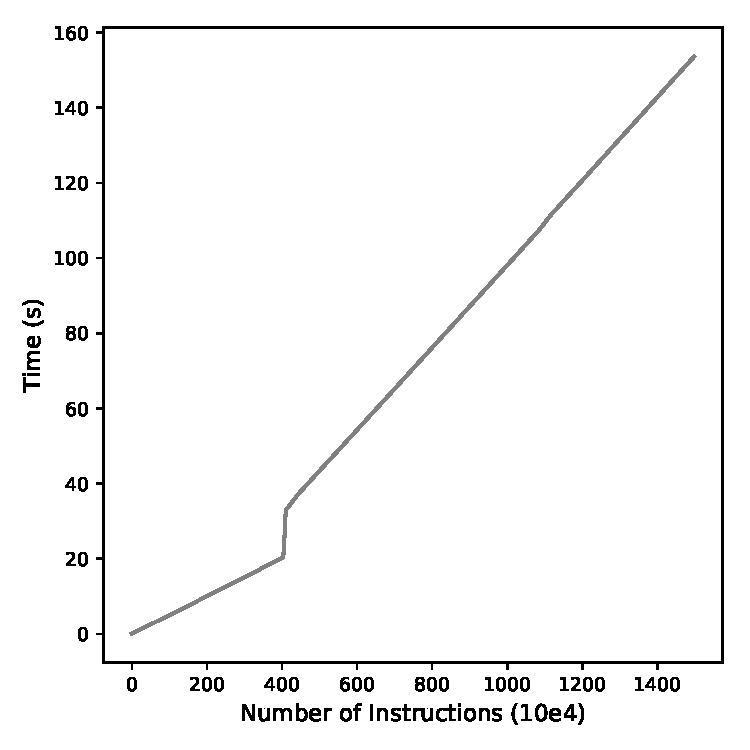
\includegraphics[width=.8\columnwidth]{./figures/result/running_time.pdf}
%    \caption{With the optimization introduced, \tool{} can be scalable to RSA}
%\end{figure}

%\subsubsection{Comparison with the Existing Tools}
\tool{} is designed to quantify side-channel leakages. But it can detect
side-channels leakages as well. In this section, we compare \tool{} with the
existing trace-based side-channel detection tools.

As shown in Table~\ref{eval:cacheD},
\tool{} not only discovers all the leakage sites reported by CacheD~\cite{203878}, but also
find many new ones. CacheD fails to detect many vulnerabilities for two
reasons. First, CacheD can only detect secret-dependent memory access
vulnerabilities. But \tool{} can detect secret-dependent control-flows as well.
Second, CacheD uses some domain
knowledge to simplify symbolic execution and has to trim the traces before
processing, which does not introduce false positives, but can neglect some
vulnerabilities. The table~\ref{eval:cacheD} shows that
\tool{} is three times faster than CacheD. As the time of symbolic execution
grow quadratically, \tool{} is much faster than CacheD when analyzing the same
number of instructions. For example, when we test~\tool{} on AES from OpenSSL
0.9.7, ~\tool{} is over %more than
100x faster than CacheD.

Since DATA~\cite{217537} need to compare several execution traces to identify
side-channel leakages, \tool{} also outperforms DATA in terms of performance.
For example, it takes 234 minutes for DATA to analysis the RSA of implementation
in OpenSSL 1.1.0f. \tool{} only spends 34 minutes according to Table~\ref{table:over_result}.
Also, DATA reports report 278 control-flow and 460 data leaks. Among those leakages,
they found two vulnerabilities. On the contrary, \tool{} can report how many bits is
actually leaked for each vulnerability, which eases the pain to identify real sensitive leaks.

\begin{table}[]
    \caption{Comparison with CacheD}
    \label{eval:cacheD}
    \vspace*{-9pt}
    \resizebox{\columnwidth}{!}{%
        \begin{tabular}{c|c|c|c|ccc}
            \hline
            \multicolumn{1}{l|}{} & \multicolumn{2}{c|}{Number of Instructions} & \multicolumn{2}{c|}{Time (s)} & \multicolumn{2}{c}{Number of Leakages}                                                                                         \\ \cline{2-7}
            \multicolumn{1}{l|}{} & \multicolumn{1}{c|}{CacheD}                 & \multicolumn{1}{c|}{\tool}    & \multicolumn{1}{c|}{CacheD}            & \multicolumn{1}{c|}{\tool}  & \multicolumn{1}{c|}{CacheD} & \multicolumn{1}{c}{\tool} \\ \hline
            AES 0.9.7             & 791                                         & 1,704                         & 43.4                                   & \multicolumn{1}{c|}{0.30}   & \multicolumn{1}{c|}{48}     & 75                        \\
            AES 1.0.2f            & 2,410                                       & 1,350                         & 48.5                                   & \multicolumn{1}{c|}{0.08}   & \multicolumn{1}{c|}{32}     & 88                        \\
            RSA 0.9.7             & 674,797                                     & 16,980,109                    & 199.3                                  & \multicolumn{1}{c|}{1681}   & \multicolumn{1}{c|}{2}      & 105                       \\
            RSA 1.0.2f            & 473,392                                     & 14,468,307                    & 165.6                                  & \multicolumn{1}{c|}{1692}   & \multicolumn{1}{c|}{2}      & 38                        \\ \hline
            Total                 & 1,151,390                                   & 31,451,470                    & 456.8                                  & \multicolumn{1}{c|}{3373.4} & \multicolumn{1}{c|}{84}     & 317                       \\ \hline
            \multicolumn{7}{l}{\# of Instructions per second \qquad  CacheD: 2,519 \qquad \tool: 9,324}                                                                                                                                          \\ \hline
        \end{tabular}
    }
\end{table}

\subsection{Case Studies}

\subsubsection{Symmetric Ciphers: DES and AES}\label{eval:sym}
We test both DES and AES ciphers from mbed TLS and OpenSSL. Both cipher
implementations apply lookup tables, which can
speed up the calculation, but can also introduce additional side-channels
as well. During our evaluation, we find mbed TLS 2.5 and 2.15.1 have the same
implementation of AES\@ and DES\@. Therefore, our tool also provides the same 
leakage report for both
versions. A sample of the generated report can be found in the Appendix~\ref{sec:result-table}.

According to \tool{}, we find DES\@ implementations in both mbed TLS and OpenSSL have several
sensitive information leakages in the key schedule function.
However, leakages in OpenSSL are more severe. We do not see any mitigation
in the new version. We think it is not seen as worth the engineering
efforts given the life cycles of DES\@.

\tool{} shows that the AES\@ in OpenSSL 1.1.1 
has less amount of leakages compared to other versions by our tools. 
(e.g., the max leakage of AES in OpenSSL 1.1.1 is 4.4 bits, but other version
have leakages that can leak can around 10 bits.)
We find that OpenSSL 1.1.1 version 
instead uses the 1KB lookup tables with 32 bit entries like older versions, it uses a 
tables with 8 bit entries. In other words, our tools shows that lookup tables with smaller 
entries will leak less amount of information. Our tool also suggests a smaller lookup
table can mitigate side-channels vulnerabilities. For example, Shown in Appendix~\ref{mbedtls_aes},
\tool{} identify seven leakages from function \textsf{mbedtls\_internal\_aes\_decrypt}.
However, \tool{} reports leakage 1, 2, 3 leak more information
compared to leakage 4, 5, 6, 7. 
We check the source code and find leakage 1, 2,
3 use secret to access the lookup table \textsf{RT0, RT1, RT2, RT3}, which is 8K
each. On the contrary, leakage 4, 5, 6, 7 each access a smaller lookup table
(2K).


\subsubsection{Asymmetric Ciphers: RSA}\label{eval:asym}
We also evaluate \tool{} on RSA.  We find developers are more interested in 
fixing side-channel vulnerabilities for RSA implementations. 
We test five versions of OpenSSL (0.9.7, 1.0.2f, 1.0.2k, 1.1.0f, 1.1.1). The
result, as shown in Figure~\ref{fig:rsa}, indicates that the newer
version of OpenSSL leaks less amount of information compared to the previous
versions. After version 0.9.7g, OpenSSL adopts a fixed-window \textsf{mod\_exp\_mont}
implementation for RSA\@. With the new design, the sequence of squares and
multiples and the memory access patterns are independent of the secret key.
\tool{}'s result confirms the new exponentiation implementation has 
effectively mitigated most of leakages because the other four versions have fewer
leakages compared with version 0.9.7. 
OpenSSL version 1.0.2f, 1.0.2k and 1.1.0f almost have the
same amount of leakage. We check the changelog and find only one change for
patching the vulnerability CVE-2016-0702. 
\tool{} find OpenSSL 1.1.1 version has significantly less amount of 
leaked information compared to other versions.
We check the changelog of OpenSSL 1.1.1 and find it claims
the new RSA implementation adopted ``numerous side-channel attack mitigation.'', 
which proves the effectiveness of our quantifying method.

\begin{figure*}
    \centering
    \vspace*{-9pt}
    \hspace*{-8pt}
    \subfloat[RSA OpenSSL 0.9.7]{
        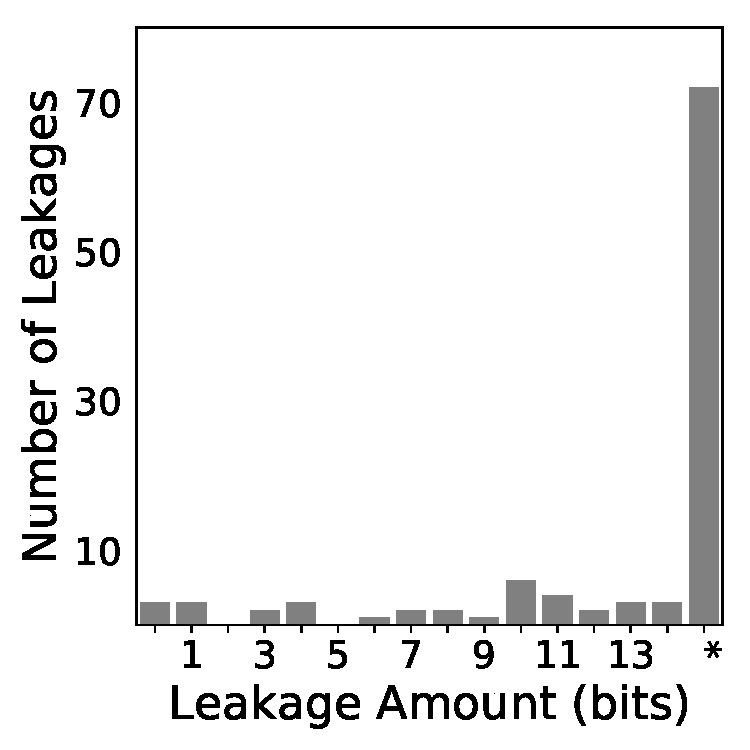
\includegraphics[width=.19\linewidth]{./figures/result/RSA-openssl-0-9-7.pdf}
        \label{fig:rsa-1}
    }
    \subfloat[RSA OpenSSL 1.0.2f]{
        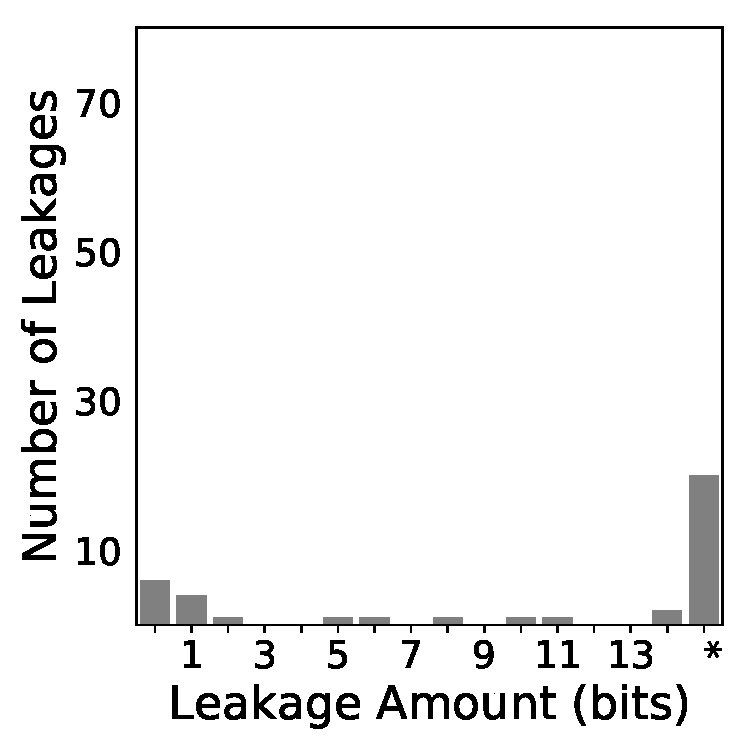
\includegraphics[width=.19\linewidth]{./figures/result/RSA-openssl-1-0-2f.pdf}
        \label{fig:rsa-2}
    }
    \subfloat[RSA OpenSSL 1.0.2k]{
        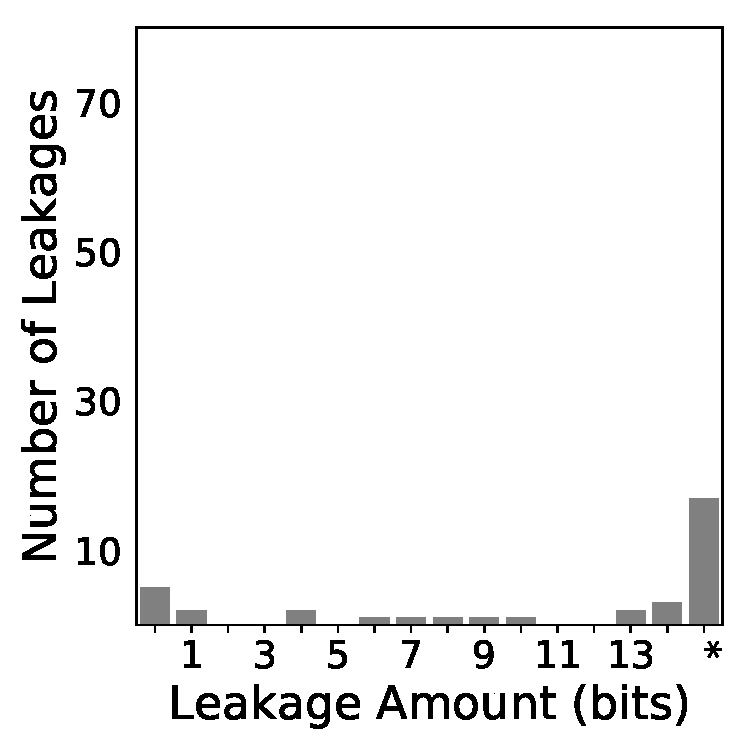
\includegraphics[width=.19\linewidth]{./figures/result/RSA-openssl-1-0-2k.pdf}
        \label{fig:rsa-3}
    }
    \subfloat[RSA OpenSSL 1.1.0f]{
        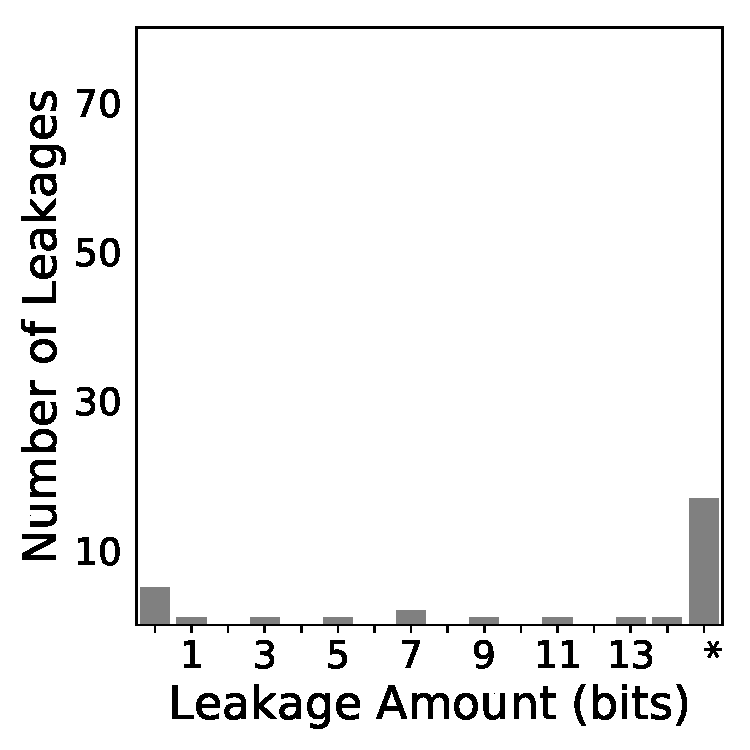
\includegraphics[width=.19\linewidth]{./figures/result/RSA-openssl-1-1-0f.pdf}
        \label{fig:rsa-4}
    }
    \subfloat[RSA OpenSSL 1.1.1]{
        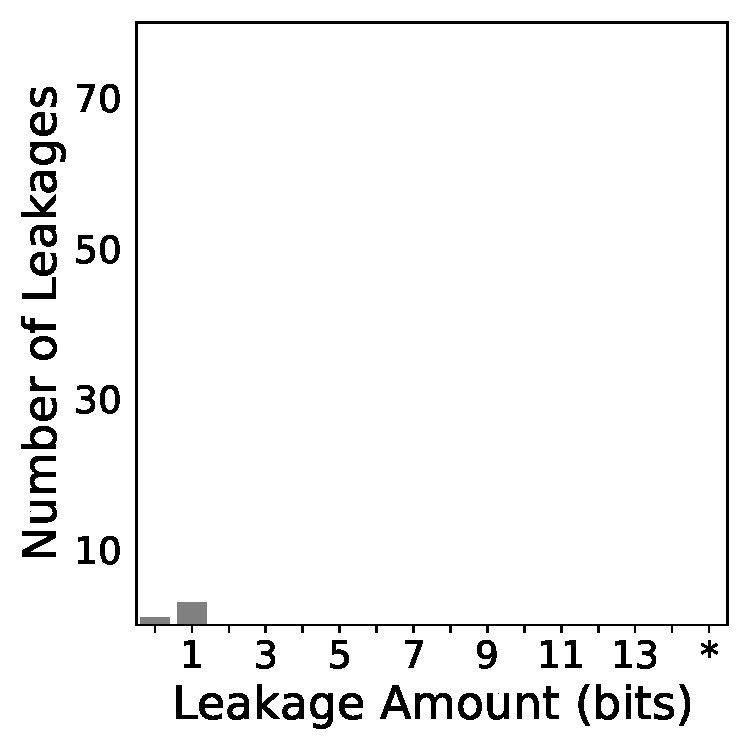
\includegraphics[width=.19\linewidth]{./figures/result/RSA-openssl-1-1-1.pdf}
        \label{fig:rsa-5}
    }
    \caption{RSA implementations in different versions of OpenSSL\@. 
        We round the number of leaked information into the nearest integer. 
        The mark $*$ means timeout,
        which indicates more severe leakages (see \S\ref{loc:timeout}).}
    \label{fig:rsa}
    \vspace*{-12pt}
\end{figure*}

Our quantification result shows vulnerabilities
that leak more information identified by \tool{} 
are more likely to be fixed in the updated version.
As presented in Figure~\ref{fig:rsa}, 
OpenSSL 0.9.7 has several severe leaks from
function \textsf{bn\_sqr\_comba8}, which is a main 
component of the OpenSSL big number implementation.
Shown in Figure~\ref{fig:old_sqr2}, it has a 
secret-dependent control flow at line 8.
The value of the function parameter \textbf{a} is derived from
the secret key. 
As function \textsf{bn\_sqr\_comba8}
calls the macro (\textsf{sqr\_add\_c2}) multiple times, 
and the code can leak some information each times.
\tool{} thinks the vulnerability is quite serious. 
The vulnerability has been patched in OpenSSL 1.1.1. Seen in 
Figure~\ref{fig:new_sqr2}, control-flows transfers are replaced. 
So there is no leaks in the function
\textsf{sqr\_add\_c2} in OpenSSL 1.1.1. We also mention
that even line 4 and 9 in Figure~\ref{fig:old_sqr2} both have if branches.
However, it is not a secret-dependent control-flow transfers because
most compilers will use \emph{add with carry} instruction to remove the branch.
Besides, branches can also be compiled to non-branch machine instructions 
like conditional moves. Therefore, simple code reviews are not accurate
enough to detect side-channels. 

On the other hand, for those vulnerabilities that leak less information. 
Developers are more reluctant to fix them. 
For example, OpenSSL 0.9.7 adopts a fixed windows version of 
function \textsf{BN\_mod\_exp\_mont\_constime} to replace original function
\textsf{BN\_mod\_exp\_mont}.
\tool{} detects a minor vulnerability in the original function that can
leaks the last bit of the big number \textbf{m}. In the updated version,
developers make the fixed windows become the default option and rewrite most parts of the 
function. However, the vulnerability still exits in OpenSSL 1.1.1,
despite the vulnerability is blunt. Details of the 
vulnerability can been seen in Appendix\S~\ref{appendix:minor:vul}.

\begin{figure}
    \centering
    \begin{lstlisting}[xleftmargin=.02\textwidth,xrightmargin=.01\textwidth]
# define mul_add_c2(a,b,c0,c1,c2) \
    t=(BN_ULLONG)a*b; \
    tt=(t+t)&BN_MASK; \
    if (tt < t) c2++; \
    t1=(BN_ULONG)Lw(tt); \
    t2=(BN_ULONG)Hw(tt); \
    c0=(c0+t1)&BN_MASK2;  \
    if ((c0 < t1) && (((++t2)&BN_MASK2) == 0)) c2++; \
    c1=(c1+t2)&BN_MASK2; if ((c1) < t2) c2++;
\end{lstlisting}
    \vspace*{-6pt}
    \caption{Macro \textsf{sqr\_add\_c2} in OpenSSL 0.9.7}
    \label{fig:old_sqr2}
    \vspace*{-6pt}
\end{figure}



\begin{figure}
    \centering
    \begin{lstlisting}[xleftmargin=.02\textwidth,xrightmargin=.01\textwidth]
# define mul_add_c2(a,b,c0,c1,c2)      do { \
    BN_ULONG ta = (a), tb = (b);            \
    BN_ULONG lo, hi, tt;                    \
    BN_UMULT_LOHI(lo,hi,ta,tb);             \
    c0 += lo; tt = hi+((c0<lo)?1:0);        \
    c1 += tt; c2 += (c1<tt)?1:0;            \
    c0 += lo; hi += (c0<lo)?1:0;            \
    c1 += hi; c2 += (c1<hi)?1:0;            \
    } while(0)
\end{lstlisting}
    \vspace*{-6pt}
    \caption{Macro \textsf{sqr\_add\_c2} in OpenSSL 1.1.1}
    \label{fig:new_sqr2}
    \vspace*{-6pt}
\end{figure}

Even for the up-to-date version of OpenSSL, \tool{} still find several
side-channel leakages. One of the vulnerabilities has the similar leaked
branch as the one in \S~\ref{appendix:minor:vul}. However, as the branch
is inside a loop and a bit shift function causes the branch leak different
bits from the sensitive buffer. The vulnerability is far severe by our tool.
Deatails of the leak can be found in Appendix \S\ref{unknown:leak} and 
Table \ref{tab:RSAOpenSSL1.1.1}.

\subsubsection{Monocypher}\label{eval:mono}
Monocypher is a small, easy to use cryptographic library with a
comparable performance as LibSodium~\cite{libsodium} and NaCl~\cite{bernstein2012security}. 
We choose four ciphers that are 
designed to be more side-channel resistant from the library.
Because those ciphers have no 
data flow from secrets to branch conditions and load addresses.
Therefore, Monocypher should be safe under our threat models. 
 %However, we are still interested in those vulnerabilities caused
 %by compiler optimizations and implementations.
We analyze those ciphers with \tool{}, and it reports no leaks from the
implementation.
This indicates that \tool\ can be used for countermeasure confirmation.


